\documentclass[preprint,12pt]{elsarticle}

\usepackage{amsmath,amssymb}
\usepackage{booktabs}
\usepackage{graphicx}
\usepackage{multirow}
\usepackage{xcolor}
\usepackage{tabularx}
\usepackage{adjustbox}
\usepackage[colorlinks=true,linkcolor=blue,citecolor=blue,urlcolor=blue,bookmarks=true]{hyperref}

\journal{Neurocomputing}

% TODO(zenodo): placeholder DOI for the Zenodo archive of this release.
% To finalize: (1) sign in at zenodo.org, (2) Settings -> Applications -> GitHub,
% authorize the Zenodo app and enable this repository, (3) push tag v1.8.1
% (or create the deposit manually and reserve its DOI), (4) replace the
% placeholder below with the reserved DOI, (5) rebuild the PDF and Word version.
\newcommand{\zenododoi}{10.5281/zenodo.XXXXXXX}

\widowpenalty=10000
\setlength{\emergencystretch}{1.5em}
\clubpenalty=10000

\hypersetup{
    pdftitle={When Does Test-Time Ensembling Help Large Language Models? A Budget-Matched Study of Answer-Space and Prompt-Space Diversity},
    pdfauthor={Chang Tan},
    pdfsubject={Test-time ensembling for large language models},
    pdfkeywords={large language models, self-consistency, prompt ensembling, uncertainty estimation, test-time compute}
}

\begin{document}

\begin{frontmatter}

\title{When Does Test-Time Ensembling Help Large Language Models? A Budget-Matched Study of Answer-Space and Prompt-Space Diversity}

\author[inst1]{Chang Tan\corref{cor1}}
\ead{aquars43@foxmail.com}
\cortext[cor1]{Corresponding author.}
\address[inst1]{Dalian University of Technology, No. 2 Linggong Road, Ganjingzi District, Dalian 116024, Liaoning, China}

\begin{abstract}
Test-time ensembling for large language models draws diversity from two sources: resampling the stochastic decoder on a fixed prompt (answer space) or aggregating semantically equivalent paraphrases (prompt space). We compare them budget-matched, answering every question sixteen times per model. A development suite (90 questions, six systems) fixed the conditions; the primary evidence is a held-out suite of 119 fresh questions fully covered by four models from two families (476 model--question pairs). Against the single-sample expectation S1, both six-vote ensembles improve out of sample: self-consistency by $+2.4$ points and the paraphrase ensemble by $+4.9$ (95\% cluster-bootstrap intervals $+1.1$ to $+3.7$ and $+2.3$ to $+7.6$), with the twelve-vote combination at $+4.1$; the two sources remain statistically inseparable ($+2.5$, interval touching zero), and $+1.9$ points of the paraphrase headline is a single-call difficulty offset, leaving $+3.0$ of within-family aggregation against $+2.4$ for resampling. The margin is conditional: it concentrates where answer-space diversity is exhausted (computation-deterministic tasks), reverses where paraphrases distort verbal-reasoning stems, and its realizing allocation is model-dependent. On saturated benchmarks, answer distributions collapse, no strategy moves accuracy, and agreement-based uncertainty estimates lose their signal. Greedy divergence from S1 is endpoint-specific (four of ten configurations). An adaptive probe-and-route rule transfers at 79--87 percent of the six-call budget, beating every fixed allocation on one model and trailing the best fixed conditions elsewhere by one to seven questions; a sequential unanimity rule preserves accuracy at two to three calls. We release prompts, paraphrases, per-call logs, and recomputation scripts.
\end{abstract}

\begin{keyword}
Large language models \sep test-time compute \sep self-consistency \sep prompt ensembling \sep uncertainty estimation \sep robustness
\end{keyword}

\end{frontmatter}

\section{Introduction}
\label{sec:intro}

Large language models answer questions through a single forward pass whose output depends on two design choices that the user controls: the prompt that specifies the task, and the decoding configuration that maps model probabilities into text. Both choices turn out to be fragile. A long line of work on prompt sensitivity shows that semantically equivalent reformulations of the same question can change model answers by large margins \citep{mizrahi2024state,sclar2024quantifying,leidinger2023language,zhu2023promptbench}. A parallel line of work on test-time compute shows that a single greedy decode is an unreliable summary of what the model knows, and that aggregating several decodes of the same prompt, as in self-consistency \citep{wang2023selfconsistency}, improves reasoning accuracy at the cost of additional inference calls.

These two observations motivate two different ways of spending a fixed budget of model calls. The first spends the budget on the answer space: keep the prompt fixed, sample several decodes at nonzero temperature, and aggregate them by majority vote. The second spends the budget on the prompt space: keep decoding deterministic or lightly stochastic, present several semantically equivalent paraphrases of the task, and aggregate the resulting answers. Both strategies are used in practice, both appear in the evaluation literature under separate headings, and both consume the same scarce resource. Surprisingly, the literature offers little guidance on which source of diversity yields more accuracy per call, whether the two sources detect the same errors, and how the answer changes with model capability and task difficulty.

The question is becoming more urgent as model behavior shifts. Post-trained flagship models are increasingly confident: on many legacy benchmarks they answer near ceiling, and preliminary reports suggest that repeated sampling at moderate temperature often returns identical answers, which would render answer-space ensembling inert precisely where deployments are most common. At the same time, uncertainty estimation methods built on sampling, such as semantic entropy \citep{kuhn2023semantic,farquhar2024detecting}, implicitly assume that the sample distribution carries information about correctness. If that assumption fails for confident models, practitioners need to know before they build on it.

This paper presents, to our knowledge, the first budget-matched, within-question comparison of answer-space and prompt-space ensembling across multiple model families and task types. Every question in our protocol is answered sixteen times by every model under matched conditions: one greedy decode, six stochastic decodes of the original prompt, one stochastic decode of each of six validated paraphrases, and three additional second decodes that support a hybrid condition. From this single call matrix we derive self-consistency ensembles of any size up to six, paraphrase ensembles of the same sizes, a hybrid allocation, a combined twelve-vote ensemble, per-question consistency scores for both diversity sources, and fragility measures that record how often paraphrasing alone flips the majority answer. Three follow-up conditions then isolate the factors the matrix alone cannot separate: a greedy-paraphrase control that removes decoding stochasticity from the paraphrase side, a chain-of-thought variant that changes the answering mode, and a hard-task probe on MMLU-Pro. Because all conditions are derived from matched calls, comparisons between strategies hold the question, the model, and the total call budget constant by construction.

Our study addresses four research questions. First, under equal budgets, does spending calls on paraphrases buy more, equal, or less accuracy than spending them on resampling, and does the hybrid allocation dominate either pure strategy? Second, how brittle are model answers to paraphrasing per se, and where do paraphrase-induced flips concentrate? Third, can agreement across paraphrases serve as an error signal in the way that agreement across samples does, and how do the two signals compare when both are available? Fourth, how do all of these effects interact with model capability and task difficulty? The last question turns out to govern the first three.

The empirical picture that emerges has a clear regime structure. When a model finds a task easy, its answer distribution collapses: across our six benchmarks, flagship models return the same answer for essentially every sample and every paraphrase on saturated tasks, self-consistency and paraphrase ensembling both collapse onto the greedy baseline, and consistency scores carry no signal about which answers are wrong. When a task genuinely challenges a model, answer entropy reappears, both ensemble families improve over greedy decoding, the two consistency measures flag partially disjoint errors, and a hybrid allocation protects against a failing diversity source. This structure implies that no single published claim about ensembling generalizes across regimes, and that practical systems should first measure the cheap statistics that identify the regime before choosing how to spend their budget.

Our contributions are as follows. We formalize test-time ensembling as a choice between two diversity sources under a shared budget, and we introduce a call matrix design that derives all conditions of interest from one matched set of calls, with controls that separate prompt-space effects from decoding stochasticity, answering mode, and task difficulty. We provide a multi-model, multi-benchmark empirical map of when each source helps, including systematic evidence that paraphrase agreement functions as an uncertainty signal whose error coverage only partially overlaps that of sample agreement. We document the answer degeneracy phenomenon that renders both ensembling and consistency-based uncertainty estimation inert on saturated tasks for confident models, with direct implications for sampling-based confidence estimation in this regime. Finally, we translate the findings into an adaptive allocation rule validated by simulation, and we release our complete prompt materials, validated paraphrases, and per-call predictions.

The remainder of the paper is organized as follows. Section~\ref{sec:related} reviews related work. Section~\ref{sec:method} formalizes the ensembling framework and the protocol. Section~\ref{sec:setup} describes models, benchmarks, and validation procedures. Section~\ref{sec:results} presents the results around our four research questions. Section~\ref{sec:discussion} discusses implications and limitations, and Section~\ref{sec:conclusion} concludes.

\section{Related Work}
\label{sec:related}

\subsection{Test-time compute and self-consistency}

Scaling computation at inference time has become a standard tool for improving the reliability of large language models. Chain-of-thought prompting demonstrates that eliciting intermediate reasoning steps raises accuracy on arithmetic and symbolic tasks \citep{wei2022chain}, and self-consistency extends this observation by sampling multiple reasoning paths at nonzero temperature and returning the most frequent final answer \citep{wang2023selfconsistency}. Follow-up work reduces the number of samples needed through early stopping \citep{aggarwal2023lets}, generalizes aggregation to free-form generation by letting the model itself select among candidate answers \citep{chen2023universal}, and studies the optimal allocation of test-time compute relative to model size \citep{snell2024scaling}. Process reward models that score intermediate steps represent a further refinement of the same budget idea \citep{lightman2023lets}. Multi-agent debate aggregates answers across multiple model instances and rounds \citep{du2023improving}, and controlled comparisons find that debate does not reliably outperform self-consistency at matched budgets \citep{smit2024mad}, which reinforces the need for budget-matched comparisons when evaluating aggregation strategies. Our work differs from this literature in the source of diversity it studies: instead of asking how many samples to draw or how to weight them, we ask whether the same calls are better spent perturbing the prompt, and we answer under a matched-budget protocol.

\subsection{Prompt sensitivity and prompt ensembling}

A separate literature documents that model outputs are sensitive to semantically irrelevant details of the prompt. Reformatting alone, such as changing spacing or option ordering, shifts accuracy by several points \citep{sclar2024quantifying}, and the measured performance of a model depends strongly on which of many equivalent prompts an evaluator happens to choose \citep{mizrahi2024state}. Linguistic properties of the prompt, such as lexical familiarity, partially predict its success \citep{leidinger2023language}, and adversarial prompt perturbations can degrade performance further \citep{zhu2023promptbench}. The natural constructive response is to aggregate over prompts. Ask Me Anything generates many question reformulations with a language model and combines the resulting pseudo-labels \citep{arora2023ask}, an idea that predates and parallels self-consistency but targets zero-shot classification rather than matched-budget reasoning. Evaluation studies propose averaging over prompt templates to stabilize benchmark scores \citep{mizrahi2024state}. What remains missing is a direct comparison that holds the budget, the model, and the question fixed and contrasts prompt-space aggregation with answer-space aggregation on the same instances, which is the gap our protocol fills.

\subsection{Uncertainty estimation from sampled behavior}

Between the two aggregation literatures sits a third that uses sampling not to improve accuracy but to estimate uncertainty. Verbalized confidence asks the model to state a probability \citep{tian2023just,xiong2024can}, and self-probing methods ask the model to evaluate its own candidate answers \citep{kadavath2022language}. Behavioral methods infer uncertainty from the dispersion of sampled outputs, from simple answer agreement to semantic clustering that treats paraphrased answers as equivalent \citep{kuhn2023semantic,farquhar2024detecting}, with surveys consolidating the rapidly growing set of measures \citep{lin2024uncertainty}. Calibration metrics such as expected calibration error \citep{guo2017calibration} and selective prediction metrics such as the area under the risk-coverage curve quantify how well a confidence score ranks correct above incorrect answers. These methods inherit an assumption from sampling: that the sample distribution is informative. Our study tests this assumption directly, characterizes the regimes in which sample agreement and paraphrase agreement carry signal, and shows that the two agreement signals are complementary where both vary. In this sense our fragility analysis also connects to work on the faithfulness of chain-of-thought explanations, which finds that stated reasoning does not always cause the final answer \citep{lanham2023measuring}: paraphrase stability measures the robustness of the answer to surface form rather than to the reasoning trace.

\subsection{Positioning}

In summary, answer-space ensembling, prompt-space ensembling, and sampling-based uncertainty estimation have developed largely in isolation. Answer-space methods assume resampling generates useful diversity. Prompt-space methods assume paraphrases probe the same knowledge. Uncertainty methods assume sample dispersion tracks correctness. All three assumptions are regime dependent, and no prior work, to our knowledge, measures all three under a single matched-budget protocol on modern models. The comparison also carries practical weight for evaluation practice, since benchmark conclusions about model capability shift when prompts vary \citep{mizrahi2024state} and when aggregation is applied \citep{wang2023selfconsistency}. Our contribution is the unified empirical map, the validation machinery for paraphrases, and the decision guidance that follows from the regime structure.

\section{A Budget-Matched Framework for Test-Time Ensembling}
\label{sec:method}

\subsection{Setup and notation}

Let $M$ denote a large language model and let $q$ denote a question with a gold answer $y^*(q)$. For multiple-choice tasks the answer is an option letter, and for free-form numeric tasks the answer is a value compared numerically. A prompt $x$ is a rendering of $q$ into natural language, consisting of an optional passage, a question stem, an option list, and an instruction that specifies the required output format. We distinguish one canonical prompt $x_0$ and $K$ paraphrased prompts $x_1, \dots, x_K$ that preserve the semantics of $x_0$ under a validation procedure described in Section~\ref{sec:setup}.

The model produces an answer through stochastic decoding. We write $a(M, x, s)$ for the answer extracted from the $s$-th independent decode of prompt $x$ at temperature $\tau = 0.7$, and $a_g(M, x)$ for the greedy decode at $\tau = 0$. Answers are extracted from the model output by a fixed parser that searches for the mandated answer format and falls back to pattern matching over the final output lines; the parse rate is reported in Section~\ref{sec:results}.

\subsection{The call matrix}

For every question and model we collect a matrix of sixteen calls:
\begin{equation}
\mathcal{C}(M, q) \;=\; \bigl\{ a_g(M, x_0) \bigr\} \;\cup\; \bigcup_{s=1}^{S} \bigl\{ a(M, x_0, s) \bigr\} \;\cup\; \bigcup_{k=1}^{K} \bigl\{ a(M, x_k, s) : s \le r_k \bigr\},
\label{eq:matrix}
\end{equation}
with $S = 6$ samples on the canonical prompt, $K = 6$ paraphrases, and $r_k = 2$ decodes for the first three paraphrases and $r_k = 1$ for the remaining three. The matrix therefore contains one greedy call, six canonical samples, six first-decode paraphrase calls, and three second-decode paraphrase calls. Every experimental condition studied in this paper is a deterministic function of this matrix, which guarantees that all comparisons hold the question, the model, and the realized decoding randomness constant across conditions.

\subsection{Ensemble conditions}

All conditions aggregate votes by majority rule. Ties are broken in favor of the earliest vote in a fixed canonical order, which prefers the canonical prompt over paraphrases and earlier paraphrases over later ones; we report tie incidence, which is negligible except where noted.

The \emph{self-consistency} condition of size $k$ aggregates the first $k$ canonical samples:
\begin{equation}
\mathrm{SC}\text{-}k(q) \;=\; \operatorname*{majority}\bigl( a(M, x_0, 1), \dots, a(M, x_0, k) \bigr), \qquad k \le 6 .
\end{equation}
The \emph{paraphrase ensemble} of size $k$ aggregates one decode of each of the first $k$ paraphrases:
\begin{equation}
\mathrm{PE}\text{-}k(q) \;=\; \operatorname*{majority}\bigl( a(M, x_1, 1), \dots, a(M, x_k, 1) \bigr), \qquad k \le 6 .
\end{equation}
Both conditions spend exactly $k$ model calls and differ only in where the diversity comes from: $\mathrm{SC}\text{-}k$ perturbs the decoder while the prompt is fixed, whereas $\mathrm{PE}\text{-}k$ perturbs the prompt while the decoder configuration is fixed. This is the budget match that makes the two conditions comparable.

The \emph{hybrid} condition splits a budget of six calls between the two sources, using two decodes of each of the first three paraphrases:
\begin{equation}
\mathrm{HB}\text{-}6(q) \;=\; \operatorname*{majority}\bigl( a(M, x_k, s) : k \in \{1,2,3\},\ s \in \{1,2\} \bigr).
\end{equation}
Finally, the \emph{combined} condition aggregates all twelve stochastic votes available in the matrix, $\mathrm{COMB}\text{-}12(q) = \operatorname{majority}\bigl( \mathrm{SC}\text{-}6(q) \cup \mathrm{PE}\text{-}6(q) \bigr)$, and serves as a twelve-call reference point for the marginal value of doubling the budget. The greedy decode $a_g(M, x_0)$ serves as the single-call baseline.

\subsection{Consistency, entropy, and fragility}

Three per-question statistics summarize the answer distribution. \emph{Sample agreement} is the frequency of the modal answer among the six canonical samples,
\begin{equation}
c_{\mathrm{S}}(q) \;=\; \max_{v} \frac{1}{6} \sum_{s=1}^{6} \mathbb{1}\bigl[ a(M, x_0, s) = v \bigr],
\end{equation}
and \emph{paraphrase agreement} $c_{\mathrm{P}}(q)$ is defined analogously over the six first-decode paraphrase answers. Both lie in $(0, 1]$, and the value $1$ indicates that the corresponding source produced no diversity at all, a situation we call \emph{answer degeneracy}. The \emph{normalized answer entropy} is the Shannon entropy of the empirical answer distribution over the twelve stochastic votes divided by its maximum possible value.

\emph{Fragility} captures disagreement between the two views of the same question: a question is fragile for a model when the majority answer of the canonical samples differs from the majority answer of the paraphrase answers, that is, when $\mathrm{SC}\text{-}6(q) \ne \mathrm{PE}\text{-}6(q)$. Fragility measures how much of the model's answer is an artifact of the particular surface form of the prompt rather than of the underlying question.

\subsection{Error detection and selective prediction}

We evaluate consistency scores as unsupervised error detectors. For each model, the consistency score of a question (reversed, so that lower agreement indicates higher predicted risk) ranks questions, and we compute the area under the receiver operating characteristic curve (AUROC) for predicting whether the reference answer is incorrect, where the reference is the combined twelve-vote ensemble unless stated otherwise. We complement AUROC with risk-coverage curves that plot the error rate of the accepted subset as the acceptance threshold varies, summarized by the area under the risk-coverage curve (AURC), and with the oracle-excess AURC (E-AURC), which measures the gap to the best achievable ranking \citep{guo2017calibration,lin2024uncertainty}. Where a model produces zero errors or constant scores on a dataset, AUROC is undefined and we report the regime instead.

\subsection{Statistical analysis}

Accuracy comparisons between two conditions on the same questions are paired by construction. We report bootstrap 95\% confidence intervals for accuracy differences (10,000 resamples, resampling questions) and two-sided exact McNemar tests for paired correctness indicators. Because models differ in the number of questions they completed within our access constraints, per-model analyses use each model's own completed question set, and pooled analyses use the intersection set, with the sample size stated in every table. We treat question sets as fixed and do not extrapolate beyond the measured benchmarks.

\section{Experimental Setup}
\label{sec:setup}

\subsection{Benchmarks}

We assemble a six-benchmark suite that spans knowledge, commonsense, mathematical reasoning, and logical reasoning, with a mix of option counts and answer formats. TruthfulQA-MC1 \citep{lin2022truthfulqa} contributes adversarial factual questions with four or five options; we shuffle option order per question to avoid position bias. PIQA \citep{bisk2020piqa} contributes two-choice physical commonsense problems. LogiQA \citep{liu2020logiqa} contributes four-choice logical reading comprehension. LSAT logical reasoning and SAT mathematics, both from the AGIEval suite \citep{zhong2023agieval}, contribute five-choice analytical reasoning and four-choice quantitative items respectively. GSM8K \citep{cobbe2021training} contributes free-form grade-school mathematics problems answered with chain-of-thought reasoning and a final numeric value. We sample fifteen questions per benchmark uniformly at random with a fixed seed, giving ninety questions in total. The mixture is deliberately diverse in difficulty: as Section~\ref{sec:results} shows, the strongest models in our pool saturate five of the six benchmarks while all models find LogiQA and, for some models, GSM8K and SAT mathematics challenging, which supplies both the degenerate and the high-entropy regimes that our analysis requires.

\subsection{Models}

We study six commercial models from four families, accessed through three providers under their free tiers: Qwen3.8-Max and Qwen3.8-Omni-Flash from the Qwen family \citep{qwen2024qwen}; Agnes3.0-Flash and Agnes2.5-Flash from the Agnes family; GPT-6-Luna from the GPT family \citep{openai2023gpt4}; and Gemini3.8-Flash from the Gemini family. The models span a range of capability tiers and post-training styles, including one model that emits an explicit private reasoning trace and one multimodal variant. All models are queried through OpenAI-compatible endpoints between October 16 and October 19, 2026. Sampling uses temperature $0.7$ with default nucleus probability; greedy calls use temperature $0$. For the two Qwen models we disable the proprietary thinking mode on multiple-choice tasks to control token expenditure and enable it on GSM8K, where chain-of-thought is necessary; all other models run in their default configurations, and every model receives the identical instruction format described below.

\subsection{Prompt design and paraphrase generation}

The canonical prompt for a multiple-choice question consists of the passage when present, the question stem, the option list labeled $(A)$ through $(E)$, and a fixed instruction that requires a direct answer in the form \texttt{Answer: <letter>} without explanation. GSM8K prompts instead require step-by-step reasoning ending with \texttt{Answer: <number>}. Direct answering on multiple-choice tasks keeps the comparison uniform across models, keeps token costs bounded, and isolates the aggregation question from chain-of-thought length effects; the GSM8K condition covers the reasoning-trace regime.

Paraphrases target the parts of the prompt where semantic-preserving variation is well defined: the question stem for TruthfulQA, LSAT, and LogiQA, and the instruction wording for GSM8K, PIQA, and SAT mathematics, whose stems contain problem-specific content such as numbers that should not be altered. This design yields two paraphrase loci, and we treat the locus as a factor in the analysis. Stem paraphrases are generated by a seventh model (Qwen3.7-Flash) that is not part of the evaluation pool, prompted to rewrite each stem in six ways while preserving all facts, entities, numbers, and the question type. Instruction paraphrases are six handcrafted variants per dataset that vary wording while keeping the literal answer-format requirement fixed, which keeps answer extraction reliable.

Every generated paraphrase passes a three-stage validation filter. A lexical stage rejects paraphrases that are identical to the original or whose length ratio falls outside $[0.4, 2.5]$. A semantic stage embeds the original stem and each candidate with a text embedding model and rejects candidates whose cosine similarity to the original falls below $0.75$. A form stage, applied to factual questions, rejects rewrites that change the question type, for example from a wh-question to a yes-no question. Candidates that fail any stage are replaced by regenerated candidates until six valid paraphrases per question are obtained; the final set achieves a mean embedding similarity of $0.86$ with the originals.

\subsection{Execution and quality control}

The experiment executes the sixteen-call matrix of Section~\ref{sec:method} for every question and model through an asynchronous runner with per-provider rate limiting, automatic retry with exponential backoff, and append-only checkpointing. Answer extraction uses the mandated \texttt{Answer:} format first and falls back to scanning the final output lines for a well-formed option letter or number, with the option range constrained by the question. Every stored record includes the extracted answer, its correctness, token usage, and a content snippet for auditing. Extraction succeeds on over 96\% of calls for every model reported in this paper; failed extractions are excluded from the corresponding question's conditions, and questions with any missing cell are excluded from that model's analysis, so all reported accuracies are computed over complete question matrices. Per-model completed question counts, which vary between 25 and 90 owing to provider rate limits, are stated alongside every result, and pooled analyses use the intersection of completed questions across the models involved.

\subsection{Conditions and metrics}

Each model and question yields the greedy baseline, $\mathrm{SC}\text{-}k$ and $\mathrm{PE}\text{-}k$ for $k \in \{2, 4, 6\}$, the hybrid $\mathrm{HB}\text{-}6$, the combined $\mathrm{COMB}\text{-}12$, the agreement statistics $c_{\mathrm{S}}$ and $c_{\mathrm{P}}$, the normalized answer entropy, and the fragility indicator. Accuracy is the fraction of questions answered correctly. Error detection is evaluated by AUROC, AURC, and E-AURC as defined in Section~\ref{sec:method}. Budget curves plot accuracy against $k$ for both pure strategies. All analysis code operates on the raw prediction logs, and we release the logs together with the prompts and paraphrases.

\section{Results}
\label{sec:results}

\subsection{Overview and data quality}
\label{sec:overview}

Table~\ref{tab:models} summarizes the six models and their completed question sets. Answer extraction succeeds on between 94.7\% and 100\% of calls across models; cells whose first decode fails to parse were re-drawn under the identical configuration until extraction succeeded, subject to provider quota. Qwen3.8-Max reached a complete sixteen-call matrix on all ninety questions; Qwen3.8-Omni reached it on seventy-one of the ninety, and the remaining four models on 12 to 40 questions each, bounded by provider rate limits and free-tier quotas. All within-model comparisons are paired and unaffected by coverage, and pooled analyses use the intersection of completed questions, stated explicitly wherever pooled numbers appear.

\begin{table}[htbp]
\centering
\small
\caption{Models, coverage, and data quality. Parse rate is the fraction of calls from which the mandated answer format was extracted after retries; $n$ is the number of questions with a complete call matrix.}
\label{tab:models}
\begin{tabular*}{\columnwidth}{@{\extracolsep{\fill}} l l l c c}
\toprule
\multicolumn{5}{l}{\textbf{Panel A: Development suite} (Oct 17--18, 2026)} \\
\midrule
Model & Family / endpoint & Tier & Parse rate & $n$ \\
\midrule
Qwen3.8-Max & Qwen / Aliyun & flagship & 99.6\% & 90 \\
Qwen3.8-Omni & Qwen / Aliyun & multimodal & 96.8\% & 71 \\
Agnes3.0-Flash & Agnes / Agnes & fast & 94.7\% & 33 \\
Agnes2.5-Flash & Agnes / Agnes & reasoning & 96.9\% & 40 \\
GPT-6-Luna & GPT / Apinex & reasoning & 100.0\% & 15 \\
Gemini3.8-Flash & Gemini / Apinex & fast & 99.6\% & 12 \\
\midrule
\multicolumn{5}{l}{\textbf{Panel B: Held-out suite} (Oct 19--23, 2026)} \\
\midrule
Model & Family / endpoint & Tier & Parse rate & $n$ \\
\midrule
Agnes3.0-Flash & Agnes / Agnes & fast & 98.7\% & 119 \\
Agnes2.5-Flash & Agnes / Agnes & reasoning & 98.1\% & 119 \\
Qwen3.7-Flash$^{\dagger}$ & Qwen / Aliyun & fast & 95.4\% & 60 \\
DeepSeekV4.1-Flash$^{\ddagger}$ & DeepSeek / Aliyun $\to$ Apinex & fast & 99.9\% & 119 \\
DeepSeekV4-Pro-0813 & DeepSeek / Apinex & pro & 99.9\% & 119 \\
DeepSeekV4-Flash-0731$^{\S}$ & DeepSeek / Aliyun & fast & 93.1\% & 13 \\
\bottomrule
\end{tabular*}

\end{table}

The sensitivity analysis in Table~\ref{tab:models} addresses the residual exclusions from two directions. Under a lenient aggregation rule that admits any question with at least four parsed votes per source, the ordering of conditions is preserved for every model: Agnes3.0-Flash moves from 78.8\% greedy to 88.1\% under SC-6 and 92.3\% under PE-6 on the extended set, and the flagship accuracies shift by at most one question. Comparing excluded with included questions on greedy accuracy shows that the excluded sets are not systematically easier: for Qwen3.8-Omni the excluded questions are nine points \emph{harder} (84.2\% versus 93.0\%), for Agnes2.5-Flash they are thirty points harder (60.0\% versus 90.0\%), while for GPT-6-Luna and Gemini3.8-Flash the few excluded questions happened to be answered correctly. The exclusions follow provider rate limits on a fixed question order rather than any adaptive choice, and both checks indicate that the complete-matrix requirement does not manufacture the effects we report.

\subsection{RQ1: Accuracy under budget-matched ensembling}
\label{sec:rq1}

Table~\ref{tab:main} reports accuracy for the five aggregation conditions together with the single-sample baseline S1, and Figure~\ref{fig:conditions} visualizes the four models with at least twenty complete questions. Two patterns dominate. First, the two Qwen flagships are at or near ceiling on five of six benchmarks, and for them the pure ensembles reproduce greedy decoding exactly: SC-6, PE-6, and COMB-12 all return 93.3\% for Qwen3.8-Max and 93.0\% for Qwen3.8-Omni, identical to greedy. The aggregation strategies are not failing; they are vacuous, because the answer distribution they aggregate contains a single value, a point that Section~\ref{sec:rq4} quantifies. Second, in the cells where models have room to err, aggregation changes answers substantially. Agnes3.0-Flash improves from 78.8\% under greedy to 90.9\% under both SC-6 and PE-6, a 12.1 point gain. Agnes2.5-Flash improves from 90.0\% to 95.0\% under SC-6 and 92.5\% under PE-6. These are large effects by the standards of inference-time methods, and they appear under both diversity sources.

\begin{table}[htbp]
\centering
\small
\caption{Main results. Accuracy (\%) under budget-matched conditions: greedy single call, single stochastic sample averaged over the six canonical draws (S1), six-vote self-consistency (SC-6), six-paraphrase ensemble (PE-6), three-paraphrase two-sample hybrid (HB-6), and the twelve-vote combined ensemble (COMB-12). Fragile is the fraction of questions whose SC-6 and PE-6 answers disagree; Degen.\ is the fraction of questions where both agreement scores equal one.}
\label{tab:main}
\scriptsize
\begin{tabular*}{\columnwidth}{@{\extracolsep{\fill}} l c c c c c c c c c}
\toprule
Model & $n$ & Greedy & S1 & SC-6 & PE-6 & HB-6 & COMB-12 & Fragile & Degen. \\
\midrule
Qwen3.8-Max & 90 & 93.3 & 93.3 & 93.3 & 93.3 & 92.2 & 93.3 & 1.1 & 97.8 \\
Qwen3.8-Omni & 71 & 93.0 & 93.9 & 93.0 & 93.0 & 91.5 & 93.0 & 4.2 & 88.7 \\
Agnes3.0-Flash & 33 & 78.8 & 89.4 & 90.9 & 90.9 & 90.9 & 90.9 & 0.0 & 75.8 \\
Agnes2.5-Flash & 40 & 90.0 & 94.2 & 95.0 & 92.5 & 92.5 & 95.0 & 2.5 & 90.0 \\
GPT-6-Luna & 15 & 80.0 & 76.7 & 73.3 & 86.7 & 86.7 & 86.7 & 13.3 & 66.7 \\
Gemini3.8-Flash & 12 & 91.7 & 86.1 & 83.3 & 91.7 & 91.7 & 91.7 & 8.3 & 66.7 \\
\bottomrule
\end{tabular*}
\end{table}

\begin{figure}[htbp]
\centering
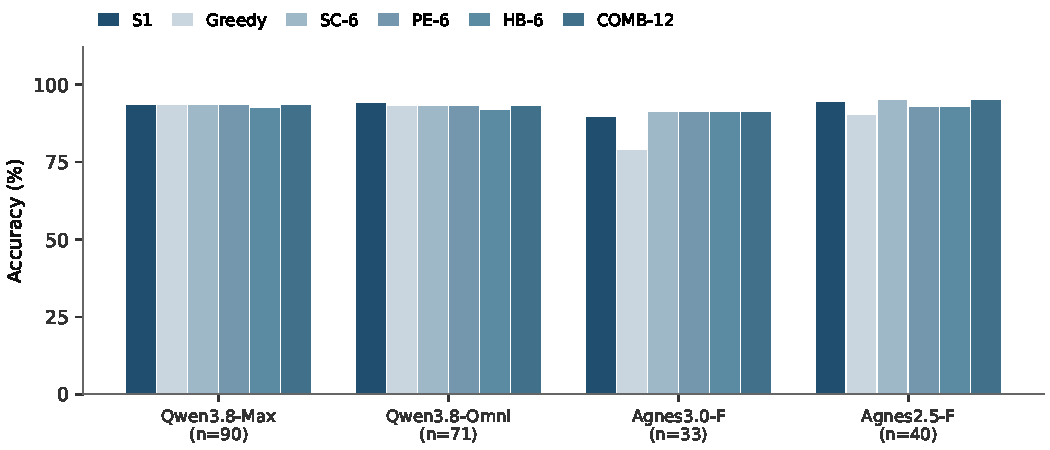
\includegraphics[width=\columnwidth]{figures/conditions.pdf}
\caption{Accuracy of the five aggregation conditions for the four models with at least twenty complete question matrices. The two Qwen flagships show identical accuracy across the pure and combined conditions, which reflects answer degeneracy rather than agreement between strategies; the hybrid differs from the pure conditions by at most one question.}
\label{fig:conditions}
\end{figure}

Three observations refine the single-call picture. First, greedy decoding is not interchangeable with a single stochastic draw. Pooled over the intersection of the four well-covered models (112 model-question pairs on 28 common questions), S1 reaches 96.4\% against 92.0\% for greedy: in the high-entropy cells the greedy answer is often not the typical sampled answer, and one temperature-$0.7$ draw is already four and a half points better on average, matching the full twelve-vote ensemble. The direction is model dependent, however: S1 beats greedy by 10.6 points for Agnes3.0-Flash but trails it for GPT-6-Luna and Gemini3.8-Flash, so neither baseline subsumes the other. Second, the hybrid allocation is a hedge rather than a dominant strategy. It matches the best pure strategy when one source fails, as for GPT-6-Luna where SC-6 loses 6.7 points while HB-6 gains 6.7, but it never exceeds the better pure strategy on any model, and it trails it by exactly one question on Qwen3.8-Max (92.2 versus 93.3), Qwen3.8-Omni (91.5 versus 93.0), and Agnes2.5-Flash (92.5 versus 95.0). Third, the twelve-vote combined ensemble does not dominate the six-vote conditions either: pooled, it reaches 96.4\% against 97.3\% for SC-6, because the paraphrase votes it adds are individually less accurate for these models and dilute the majority. Doubling the budget therefore buys no guarantee; vote quality governs the marginal value of additional votes.

On the central question, whether one diversity source buys more accuracy per call than the other, we detect no difference: pooled over the same 112 pairs, SC-6 gains 5.4 points over greedy and PE-6 gains 3.6, the SC-6 advantage is 1.8 points, and no per-model McNemar test approaches significance (all $p \ge 0.5$; Table~\ref{tab:tests}). We emphasize what this does and does not establish. The question-level cluster bootstrap interval for the pooled SC-6 advantage is $[0.0, 5.4]$ points, and the TOST procedure at equivalence bounds of $\pm 3$ points does not conclude equivalence for the pooled difference, nor for the models with small completed sets. At these sample sizes the study is powered to detect only large differences; a genuine advantage of either source of up to several points could go unnoticed. The two strategies are therefore not interchangeable in principle, and for two reasons the data show they are not interchangeable in practice either: they disagree on individual questions at measurable rates (Section~\ref{sec:rq2}), and their agreement signals catch different errors (Section~\ref{sec:rq3}).

\begin{table}[htbp]
\centering
\footnotesize
\caption{Paired comparisons between conditions: discordant counts ($b$: first condition right, second wrong; $c$: the reverse), exact McNemar $p$, accuracy difference with 95\% question-resampled bootstrap CI, and the TOST verdict at $\pm 3$ point equivalence bounds. ``no'' means equivalence is not established at this sample size, not that a difference was found.}
\label{tab:tests}
\scriptsize
\begin{tabular*}{\columnwidth}{@{\extracolsep{\fill}} l c l c c c c c c}
\toprule
Model & $n$ & Comparison & $b$ & $c$ & McNemar $p$ & Diff. & 95\% CI & TOST $\pm$3 \\
\midrule
Qwen3.8-Max & 90 & SC-6 $-$ S1 & -- & -- & -- & +0.0 & [0.0,0.0] & -- \\
 &  & PE-6 $-$ S1 & -- & -- & -- & +0.0 & [0.0,0.0] & -- \\
 &  & SC-6 $-$ Greedy & 0 & 0 & 1.000 & +0.0 & [0.0,0.0] & -- \\
 &  & SC-6 $-$ PE-6 & 0 & 0 & 1.000 & +0.0 & [0.0,0.0] & yes \\
\addlinespace
Qwen3.8-Omni & 71 & SC-6 $-$ S1 & -- & -- & -- & -0.9 & [-3.3,1.2] & -- \\
 &  & PE-6 $-$ S1 & -- & -- & -- & -0.9 & [-4.0,1.6] & -- \\
 &  & SC-6 $-$ Greedy & 1 & 1 & 1.000 & +0.0 & [-4.2,4.2] & -- \\
 &  & SC-6 $-$ PE-6 & 1 & 1 & 1.000 & +0.0 & [-4.2,4.2] & yes \\
\addlinespace
Agnes3.0-Flash & 33 & SC-6 $-$ S1 & -- & -- & -- & +1.5 & [-2.5,6.1] & -- \\
 &  & PE-6 $-$ S1 & -- & -- & -- & +1.5 & [-2.5,6.1] & -- \\
 &  & SC-6 $-$ Greedy & 4 & 0 & 0.125 & +12.1 & [3.0,24.2] & -- \\
 &  & SC-6 $-$ PE-6 & 0 & 0 & 1.000 & +0.0 & [0.0,0.0] & yes \\
\addlinespace
Agnes2.5-Flash & 40 & SC-6 $-$ S1 & -- & -- & -- & +0.8 & [0.0,2.5] & -- \\
 &  & PE-6 $-$ S1 & -- & -- & -- & -1.7 & [-5.0,0.0] & -- \\
 &  & SC-6 $-$ Greedy & 2 & 0 & 0.500 & +5.0 & [0.0,12.5] & -- \\
 &  & SC-6 $-$ PE-6 & 1 & 0 & 1.000 & +2.5 & [0.0,7.5] & no \\
\addlinespace
GPT-6-Luna & 15 & SC-6 $-$ S1 & -- & -- & -- & -3.3 & [-12.2,4.4] & -- \\
 &  & PE-6 $-$ S1 & -- & -- & -- & +10.0 & [0.0,22.2] & -- \\
 &  & SC-6 $-$ Greedy & 0 & 1 & 1.000 & -6.7 & [-20.0,0.0] & -- \\
 &  & SC-6 $-$ PE-6 & 0 & 2 & 0.500 & -13.3 & [-33.3,0.0] & no \\
\addlinespace
Gemini3.8-Flash & 12 & SC-6 $-$ S1 & -- & -- & -- & -2.8 & [-12.5,4.2] & -- \\
 &  & PE-6 $-$ S1 & -- & -- & -- & +5.6 & [0.0,13.9] & -- \\
 &  & SC-6 $-$ Greedy & 0 & 1 & 1.000 & -8.3 & [-25.0,0.0] & -- \\
 &  & SC-6 $-$ PE-6 & 0 & 1 & 1.000 & -8.3 & [-25.0,0.0] & no \\
\bottomrule
\end{tabular*}
\end{table}

The comparison is also matched in tokens, not only in calls. Averaged per call, canonical-sample and paraphrase calls cost within one to five percent of each other for every model (for example 223 versus 219 tokens for Qwen3.8-Max and 505 versus 528 for GPT-6-Luna), because validated paraphrases change the surface form but not the length of the task: the mean character-length ratio between paraphrase and original stems is 1.06 for the Qwen models and 1.13 to 1.14 for the API-served models. Budgets matched in calls are therefore approximately matched in cost for this suite.

\subsection{RQ2: Paraphrase fragility}
\label{sec:rq2}

Fragility, the fraction of questions where paraphrasing alone flips the majority answer, is negligible in the degenerate regime and substantial in the high-entropy regime. Qwen3.8-Max shows fragility on 1.1\% of questions and Qwen3.8-Omni on 4.2\%, concentrated almost entirely in LogiQA, where the respective per-dataset fragility rates are 6.7\% and 21.4\%. The models with high answer entropy on logical reasoning show more: GPT-6-Luna flips on 13.3\% of its questions overall and on 40\% of its LogiQA questions, and Gemini3.8-Flash on 8.3\% overall and 33.3\% of LogiQA. Agnes3.0-Flash, whose gains come with fully consistent votes across both sources, shows zero fragility.

Stratifying by paraphrase locus, as preregistered in the design, shows that flips are entirely a stem-locus phenomenon. Across all six models, no question ever flips under instruction paraphrasing (zero of 52 pooled instruction-locus pairs), while 3.3\% of pooled stem-locus pairs flip, rising to 28.6\% and 20\% for GPT-6-Luna and Gemini3.8-Flash respectively. The two loci differ by construction in how much of the prompt they vary, so the asymmetry should be read as a property of the perturbation family rather than of the models: instruction rewordings touch only the answer-format scaffolding, while stem rewordings touch the problem content itself. For evaluation practice, the practical consequence is that a single-prompt score on a hard benchmark understates the instability of the measured system by an amount that stem fragility makes visible, and that instruction-level prompt ensembling, as sometimes used to stabilize benchmark scores, probes a much weaker axis of variation than stem-level paraphrasing.

Fragility is not random noise; it tracks the same model-task cells that carry answer entropy and ensembling gains, which supports reading it as an observable symptom of unstable knowledge rather than as a formatting artifact. It is also not an artifact of loose paraphrases: recomputing the statistic with only the paraphrases whose fresh embedding similarity exceeds the stricter 0.80 threshold, requiring at least four such paraphrases per question, leaves the rates essentially unchanged or higher for every model (GPT-6-Luna 33.3\% on six qualifying questions versus 13.3\% overall; Gemini3.8-Flash 25.0\% versus 8.3\%; Qwen3.8-Omni 4.8\% versus 4.2\%), so if anything the tighter paraphrases flip more. Section~\ref{sec:greedypara} returns to fragility with a decoding-noise-free variant computed from greedy paraphrase decodes.

\subsection{RQ3: Consistency as an error signal}
\label{sec:rq3}

Table~\ref{tab:uncert} evaluates agreement scores as unsupervised detectors of ensemble errors, and Figure~\ref{fig:auroc} visualizes AUROC. Models with fewer than five ensemble errors are marked with a dagger and reported descriptively only, following the analysis plan; at one to three errors, AUROC values are dominated by individual questions and their confidence intervals would span most of the unit interval. The pattern follows the regime structure. For the Qwen flagships, where almost every question is degenerate, sample agreement carries almost no signal (AUROC 0.58 for Qwen3.8-Max, 95\% CI $[0.50, 0.78]$) because the score is constant at one for nearly all questions, right or wrong; the degenerate stratum contributes errors that are invisible to any agreement-based detector by construction, and five of Qwen3.8-Max's six errors are missed by both signals. Qwen3.8-Omni retains moderate signal (0.79). In the models with genuine entropy the scores become informative and the stronger source differs across models: for Agnes3.0-Flash, sample agreement is highly discriminative (0.96, CI $[0.89, 1.00]$) while paraphrase agreement is weak (0.60), whereas for GPT-6-Luna paraphrase agreement is the stronger signal (0.92 against 0.58) and for Gemini3.8-Flash both signals separate its single error perfectly. Agnes2.5-Flash, whose answers are mostly degenerate, shows a reversed sample-agreement ranking that we read as noise at its two-error rate.

\begin{table}[htbp]
\centering
\footnotesize
\caption{Uncertainty estimation. Error rate of the COMB-12 reference, AUROC of reversed agreement scores for predicting ensemble errors (95\% bootstrap CI where the model has at least five errors), and the area under the risk-coverage curve (AURC; lower is better, computed by accepting questions in decreasing order of confidence). Both is the sum of the two disagreement scores. $^\dagger$Fewer than five errors: descriptive only. Dashes indicate constant scores or zero errors.}
\label{tab:uncert}
\footnotesize
\begin{tabular*}{\columnwidth}{@{\extracolsep{\fill}} l c c c c c c c}
\toprule
 & & \multicolumn{3}{c}{AUROC} & \multicolumn{3}{c}{AURC} \\
\cmidrule(lr){3-5}\cmidrule(lr){6-8}
Model & Err. & $c_S$ & $c_P$ & Both & $c_S$ & $c_P$ & Both \\
\midrule
Qwen3.8-Max & 6.7 & 0.583 & 0.576 & 0.578 & 0.079 & 0.080 & 0.080 \\
Qwen3.8-Omni & 7.0 & 0.788 & 0.779 & 0.780 & 0.009 & 0.010 & 0.010 \\
Agnes3.0-Flash$^\dagger$ & 9.1 & 0.961 & 0.600 & 0.922 & 0.009 & 0.158 & 0.013 \\
Agnes2.5-Flash$^\dagger$ & 5.0 & 0.487 & 0.704 & 0.704 & 0.026 & 0.029 & 0.029 \\
GPT-6-Luna$^\dagger$ & 13.3 & 0.577 & 0.923 & 0.769 & 0.060 & 0.024 & 0.046 \\
Gemini3.8-Flash$^\dagger$ & 8.3 & 0.955 & 0.955 & 1.000 & 0.015 & 0.015 & 0.007 \\
\bottomrule
\end{tabular*}
\end{table}

\begin{figure}[htbp]
\centering
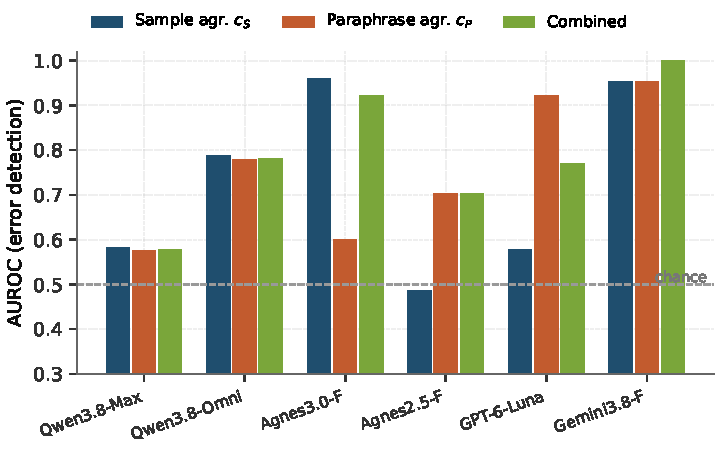
\includegraphics[width=0.8\columnwidth]{figures/auroc.pdf}
\caption{AUROC of reversed agreement scores for detecting ensemble errors. The dashed line marks chance. Signal strength follows the entropy regime, and the stronger source differs across models. $^\dagger$Models with fewer than five errors, reported descriptively.}
\label{fig:auroc}
\end{figure}

The risk-coverage analysis in Table~\ref{tab:uncert} quantifies the selective-prediction value of each signal. With the acceptance order fixed to decreasing confidence, sample agreement attains an AURC of 0.009 for Qwen3.8-Omni against an overall error rate of 7.0\%, and 0.009 for Agnes3.0-Flash against 9.1\%; paraphrase agreement attains 0.010 and 0.158 respectively, so the AURC ordering tracks the AUROC ordering, and for Qwen3.8-Max, whose signals are uninformative, AURC stays at the chance level implied by its 6.7\% error rate. Pooled over the four well-covered models, sample agreement reaches an AUROC of 0.74 (cluster-bootstrap 95\% CI $[0.71, 0.75]$) against 0.60 $[0.46, 0.73]$ for paraphrase agreement, an interval that overlaps chance: pooled across models with opposite signal strengths, the paraphrase signal averages out.

The two agreement scores therefore measure different failure modes, but the evidence for complementarity is about coverage, not about a superior combined detector. Among the ensemble errors of the models with informative signals, the flagged sets overlap only partially: for Agnes3.0-Flash, sample agreement flags all three errors while paraphrase agreement flags one, two of them only through sample agreement; for GPT-6-Luna, paraphrase agreement flags both errors and sample agreement only one; for Qwen3.8-Omni the two signals flag the same three of five errors. Accordingly, the combined Both score exceeds the best single signal only for Gemini3.8-Flash, ties it for Agnes3.0-Flash (0.92 against 0.96 for sample agreement alone, i.e., slightly below), and falls between the two singles elsewhere; pooled it reaches 0.73 against 0.74 for sample agreement alone. A deployment that can afford both probes obtains partially disjoint evidence, and neither signal subsumes the other, but summing the two disagreement scores is not the way to combine them; a learned or calibrated combination is a natural next step. We also note the structural caveat of Section~\ref{sec:method}: on questions where all twelve votes coincide, the reference answer equals that unanimous vote by construction, so detectors that read unanimity are correct by definition on the degenerate stratum; the informative content of Table~\ref{tab:uncert} lies in the non-degenerate stratum, which the flagged-error analysis above reflects.

\subsection{RQ4: The regime structure}
\label{sec:rq4}

Table~\ref{tab:regime} reports per model and dataset the greedy accuracy, the combined-ensemble accuracy, the mean answer entropy, and the degeneracy rate, and Figure~\ref{fig:regime} plots the ensemble gain against entropy for every model-dataset cell. The scatter shows the central dependency of the entire study: gains from ensembling are confined to cells with positive entropy. Across the pooled (model, question) pairs of the four well-covered models, the Spearman rank correlation between answer entropy and the COMB-12 gain over greedy is 0.62. Because the entropy and the combined ensemble share the same underlying votes, we recompute the correlation with strictly disjoint votes: entropy over the six canonical samples against the PE-6 gain gives 0.42, and entropy over the six paraphrase votes against the SC-6 gain gives 0.66. The dependency survives removing the shared-vote circularity, with the sample-side correlation somewhat stronger than the paraphrase-side one. Stratified, the dependence is stark. In the degenerate stratum, 104 of 112 pooled pairs, greedy accuracy is 97.1\% and every ensemble condition lands within 1.0 point of it. In the high-entropy stratum above 0.15, eight pooled pairs, greedy accuracy is 25.0\%, SC-6 lifts it to 87.5\%, PE-6 and the hybrid to 62.5\%, and the combined ensemble to 75.0\%.

\begin{table}[htbp]
\centering
\footnotesize
\caption{Regime map by model and dataset: greedy accuracy, COMB-12 accuracy, their difference, mean support-normalized answer entropy, and the degeneracy rate (both agreement scores equal to one).}
\label{tab:regime}
\scriptsize
\begin{tabular*}{\columnwidth}{@{\extracolsep{\fill}} l l c c c c c c c}
\toprule
Model & Dataset & $n$ & Greedy & S1 & COMB & $\Delta_C$ & Share & Diss.\% \\
\midrule
Qwen3.8-Max & GSM8K & 15 & 100.0 & 100.0 & 100.0 & +0.0 & 100.0 & 0.0 \\
Qwen3.8-Max & SAT-Math & 15 & 100.0 & 100.0 & 100.0 & +0.0 & 100.0 & 0.0 \\
Qwen3.8-Max & PIQA & 15 & 100.0 & 100.0 & 100.0 & +0.0 & 98.9 & 1.1 \\
Qwen3.8-Max & TruthfulQA & 15 & 100.0 & 100.0 & 100.0 & +0.0 & 100.0 & 0.0 \\
Qwen3.8-Max & LSAT-LR & 15 & 100.0 & 100.0 & 100.0 & +0.0 & 100.0 & 0.0 \\
Qwen3.8-Max & LogiQA & 15 & 60.0 & 60.0 & 60.0 & +0.0 & 97.2 & 2.8 \\
\midrule
Qwen3.8-Omni & GSM8K & 15 & 100.0 & 100.0 & 100.0 & +0.0 & 100.0 & 0.0 \\
Qwen3.8-Omni & SAT-Math & 1 & 100.0 & 100.0 & 100.0 & +0.0 & 91.7 & 8.3 \\
Qwen3.8-Omni & PIQA & 11 & 100.0 & 100.0 & 100.0 & +0.0 & 100.0 & 0.0 \\
Qwen3.8-Omni & TruthfulQA & 15 & 93.3 & 96.7 & 93.3 & -3.3 & 96.1 & 3.9 \\
Qwen3.8-Omni & LSAT-LR & 15 & 100.0 & 98.9 & 100.0 & +1.1 & 99.4 & 0.6 \\
Qwen3.8-Omni & LogiQA & 14 & 71.4 & 73.8 & 71.4 & -2.4 & 89.3 & 10.7 \\
\midrule
Agnes3.0-Flash & GSM8K & 7 & 85.7 & 97.6 & 100.0 & +2.4 & 94.0 & 6.0 \\
Agnes3.0-Flash & SAT-Math & 2 & 100.0 & 100.0 & 100.0 & +0.0 & 95.8 & 4.2 \\
Agnes3.0-Flash & PIQA & 5 & 100.0 & 100.0 & 100.0 & +0.0 & 100.0 & 0.0 \\
Agnes3.0-Flash & TruthfulQA & 5 & 100.0 & 100.0 & 100.0 & +0.0 & 100.0 & 0.0 \\
Agnes3.0-Flash & LSAT-LR & 6 & 83.3 & 88.9 & 83.3 & -5.6 & 95.8 & 4.2 \\
Agnes3.0-Flash & LogiQA & 8 & 37.5 & 66.7 & 75.0 & +8.3 & 84.4 & 15.6 \\
\midrule
Agnes2.5-Flash & GSM8K & 7 & 85.7 & 100.0 & 100.0 & +0.0 & 98.8 & 1.2 \\
Agnes2.5-Flash & SAT-Math & 11 & 100.0 & 100.0 & 100.0 & +0.0 & 99.2 & 0.8 \\
Agnes2.5-Flash & PIQA & 7 & 85.7 & 85.7 & 85.7 & +0.0 & 98.8 & 1.2 \\
Agnes2.5-Flash & TruthfulQA & 4 & 100.0 & 100.0 & 100.0 & +0.0 & 100.0 & 0.0 \\
Agnes2.5-Flash & LSAT-LR & 6 & 83.3 & 83.3 & 83.3 & +0.0 & 100.0 & 0.0 \\
Agnes2.5-Flash & LogiQA & 5 & 80.0 & 93.3 & 100.0 & +6.7 & 90.0 & 10.0 \\
\midrule
GPT-6-Luna & GSM8K & 1 & 100.0 & 100.0 & 100.0 & +0.0 & 100.0 & 0.0 \\
GPT-6-Luna & SAT-Math & 5 & 80.0 & 80.0 & 80.0 & +0.0 & 96.7 & 3.3 \\
GPT-6-Luna & PIQA & 2 & 100.0 & 100.0 & 100.0 & +0.0 & 100.0 & 0.0 \\
GPT-6-Luna & TruthfulQA & 2 & 100.0 & 100.0 & 100.0 & +0.0 & 100.0 & 0.0 \\
GPT-6-Luna & LogiQA & 5 & 60.0 & 50.0 & 80.0 & +30.0 & 73.3 & 26.7 \\
\midrule
Gemini3.8-Flash & GSM8K & 1 & 100.0 & 100.0 & 100.0 & +0.0 & 100.0 & 0.0 \\
Gemini3.8-Flash & SAT-Math & 4 & 100.0 & 100.0 & 100.0 & +0.0 & 93.8 & 6.2 \\
Gemini3.8-Flash & PIQA & 2 & 100.0 & 100.0 & 100.0 & +0.0 & 100.0 & 0.0 \\
Gemini3.8-Flash & TruthfulQA & 2 & 100.0 & 100.0 & 100.0 & +0.0 & 100.0 & 0.0 \\
Gemini3.8-Flash & LogiQA & 3 & 66.7 & 44.4 & 66.7 & +22.2 & 66.7 & 33.3 \\
\bottomrule
\end{tabular*}
\end{table}

\begin{figure}[htbp]
\centering
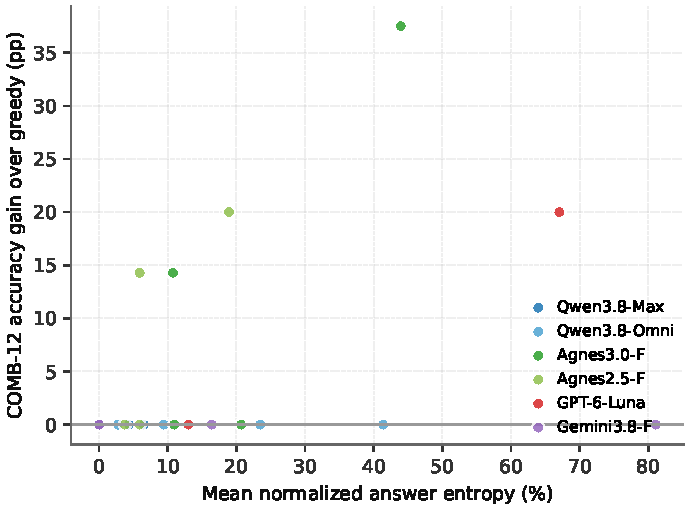
\includegraphics[width=0.75\columnwidth]{figures/regime.pdf}
\caption{Ensemble gain over greedy against mean answer entropy for every model-dataset cell. Gains concentrate where entropy is positive. The one cell with entropy above 0.8 and no combined-ensemble gain is LogiQA under Gemini3.8-Flash ($n=3$), where the modal answer is not the correct one; LogiQA under GPT-6-Luna, with entropy 0.67, gains 20 points under PE-6 and COMB-12 while losing 20 under SC-6, illustrating that the sign of the gain depends on whether the modal answer is correct, not on entropy alone.}
\label{fig:regime}
\end{figure}

Within the high-entropy region, entropy alone does not guarantee gains, and the exception is instructive. The highest-entropy cell in the study is LogiQA under Gemini3.8-Flash, entropy 0.81 with $n=3$, whose ensemble accuracy does not move. LogiQA under GPT-6-Luna, entropy 0.67 with $n=5$, shows the full regime structure in one cell: greedy answers 60\% correctly, the six-sample majority drops to 40\% because the modal sampled answer is wrong, while the paraphrase majority rises to 80\% and takes the combined ensemble with it. The plurality-vote model of Section~\ref{sec:condorcet} summarizes the pattern: entropy is a necessary condition for aggregation to matter, but the sign of the gain is determined by whether the modal answer is correct, which entropy does not measure.

The budget curves in Figure~\ref{fig:budget} complete the picture, with the single-sample baseline S1 at $k=1$ and the greedy level marked as a dotted line; panel headers state how many percentage points one question contributes, since a single flipped question moves accuracy by 1.1 to 3.0 points at these sample sizes. For the flagships the curves are flat at the greedy level within one question at every budget, with the one-question deviations reflecting individual tie-breaks rather than trends: Qwen3.8-Max dips one question under PE at $k \in \{2,4\}$, and Qwen3.8-Omni wiggles one question above greedy under SC-4. For Agnes3.0-Flash, the paraphrase ensemble reaches its full 90.9\% already at $k=2$ while the sample majority needs $k=4$ to catch up, the two curves crossing rather than one leading throughout. For Agnes2.5-Flash the ordering is the reverse and persists: sample voting climbs to 95.0\% by $k=6$ while paraphrase voting plateaus at 92.5\%. The practical reading is that the choice between the two sources matters less than the choice of whether to aggregate at all, which the entropy regime determines, and that neither source dominates the other in budget profile across models.

\begin{figure}[htbp]
\centering
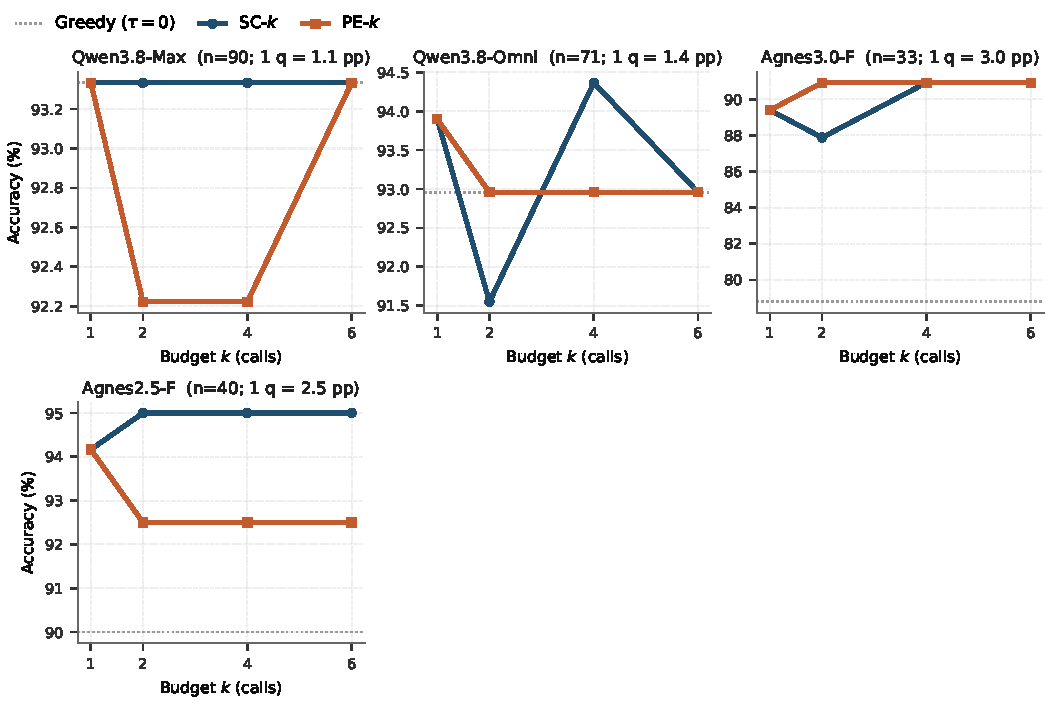
\includegraphics[width=\columnwidth]{figures/budget.pdf}
\caption{Accuracy against call budget $k$ for self-consistency (SC-$k$) and paraphrase ensembling (PE-$k$), with the single-sample baseline S1 at $k=1$ and the greedy accuracy as a dotted line. Panel headers give each model's question count and the accuracy value of one question. Flat curves indicate the degenerate regime; rising or crossing curves indicate cells where aggregation changes answers.}
\label{fig:budget}
\end{figure}

\subsection{Isolating the prompt-space effect: greedy paraphrases}
\label{sec:greedypara}

The standard paraphrase ensemble decodes each paraphrase once at $\tau = 0.7$, so its diversity mixes prompt-space variation with decoding stochasticity. The greedy-paraphrase control removes the second component by decoding each paraphrase at $\tau = 0$, yielding the noise-free ensemble $\mathrm{PE}^{g}\text{-}6$ and a fragility indicator in which neither side involves sampling. Table~\ref{tab:greedypara} reports the control for the five models whose provider quota allowed it.

\begin{table}[htbp]
\centering
\footnotesize
\caption{Greedy-paraphrase control. Accuracy (\%) of the greedy baseline, SC-6, PE-6, and the greedy-decoded paraphrase ensemble PE$^{g}$-6; Frag.$^{g}$ is the fraction of questions where SC-6 and PE$^{g}$-6 disagree (no decoding noise on the paraphrase side); Degen.$^{g}$ is the fraction of questions where all six greedy paraphrase answers coincide.}
\label{tab:greedypara}
\footnotesize
\begin{tabular*}{\columnwidth}{@{\extracolsep{\fill}} l c c c c c c c}
\toprule
Model & $n$ & Greedy & SC-6 & PE-6 & PE$^{g}$-6 & Frag.$^{g}$ & Degen.$^{g}$ \\
\midrule
Qwen3.8-Max & 88 & 93.2 & 93.2 & 93.2 & 93.2 & 1.1 & 98.9 \\
Qwen3.8-Omni & -- & \multicolumn{6}{c}{quota exhausted before the control could be run} \\
Agnes3.0-Flash & 32 & 81.2 & 93.8 & 93.8 & 93.8 & 3.1 & 71.9 \\
Agnes2.5-Flash & 39 & 89.7 & 94.9 & 92.3 & 92.3 & 2.6 & 89.7 \\
GPT-6-Luna & 15 & 80.0 & 73.3 & 86.7 & 80.0 & 40.0 & 53.3 \\
Gemini3.8-Flash & 12 & 91.7 & 83.3 & 91.7 & 83.3 & 25.0 & 41.7 \\
\bottomrule
\end{tabular*}
\end{table}

The control separates three effects. First, for the flagship, degeneracy is not a temperature artifact: 98.9\% of Qwen3.8-Max's questions return six identical answers even under greedy decoding of six different paraphrases, and $\mathrm{PE}^{g}\text{-}6$ equals PE-6, SC-6, and greedy to the question. The collapse is a property of the model-task pair, not of the sampling distribution around it. Second, for the mid-tier models, the prompt-space effect carries the paraphrase ensemble almost entirely: $\mathrm{PE}^{g}\text{-}6$ matches PE-6 to the question for Agnes3.0-Flash and Agnes2.5-Flash, so the stochastic component of PE contributes nothing beyond the paraphrases themselves in these cells. Third, for the prompt-brittle models, decoding noise and prompt variation interact: GPT-6-Luna's greedy paraphrase ensemble reaches 80.0\% against 86.7\% for the sampled version, and Gemini3.8-Flash 83.3\% against 91.7\%, so for the most fragile models the sampled paraphrase ensemble retains a two-to-eight point edge over its noise-free counterpart. Fragility itself survives the control in strengthened form: GPT-6-Luna flips on 40.0\% of questions and Gemini3.8-Flash on 25.0\% when both sides are decoded greedily, which rules out sampling noise as the cause of paraphrase-induced flips and locates the instability in the model's response to the prompt's surface form.

\subsection{Harder tasks: the MMLU-Pro probe}
\label{sec:mmlupro}

The flagship models saturate five of the six main-suite benchmarks, so the degenerate regime dominates their measurements. The MMLU-Pro probe asks whether a harder distribution restores answer entropy under the same direct-answering protocol. Table~\ref{tab:mmlupro} reports the probe; the coverage caveat is stated up front: on hard quantitative items the direct-answering instruction does not always suppress reasoning, and outputs truncated at the token cap lost extraction on a majority of Qwen3.8-Max's probe calls, leaving five complete questions (eight more with at least four parsed votes); the other models parsed cleanly.

\begin{table}[htbp]
\centering
\footnotesize
\caption{MMLU-Pro probe: greedy accuracy, single-sample accuracy S1, and SC-6 accuracy, with mean support-normalized sample entropy, sample degeneracy rate, and the model's main-suite entropy for comparison.}
\label{tab:mmlupro}
\footnotesize
\begin{tabular*}{\columnwidth}{@{\extracolsep{\fill}} l c c c c c c c}
\toprule
Model & $n$ & Greedy & S1 & SC-6 & Entropy & Degen. & Suite entropy \\
\midrule
Qwen3.8-Max & 6 & 50.0 & 50.0 & 50.0 & 0.153 & 83.3 & 0.018 \\
Agnes3.0-Flash & 8 & 12.5 & 6.2 & 0.0 & 0.937 & 0.0 & 0.162 \\
Agnes2.5-Flash & 13 & 84.6 & 76.9 & 84.6 & 0.241 & 69.2 & 0.055 \\
GPT-6-Luna & 15 & 66.7 & 66.7 & 73.3 & 0.261 & 66.7 & 0.267 \\
\bottomrule
\end{tabular*}
\end{table}

The probe shows that difficulty alone does not determine the regime. GPT-6-Luna, the strongest model with full probe coverage, lands in the high-entropy regime: greedy accuracy 66.7\% with mean entropy 0.26 and a 66.7\% degeneracy rate, and self-consistency lifts it to 73.3\%, a 6.6 point gain that mirrors the main-suite pattern for mid-tier models. Qwen3.8-Max remains essentially degenerate on the probe: its six complete questions are unanimous on five, and seven of the eight questions with at least four parsed votes return a single answer, so for this flagship a ten-option hard benchmark under direct answering still collapses to one answer per question. At the other end, Agnes3.0-Flash collapses into near-uniform guessing: entropy 0.94 with zero degeneracy, greedy accuracy 12.5\%, and a self-consistency majority of 0\%, worse than chance, exactly the plurality-vote failure mode of Section~\ref{sec:condorcet} when the modal answer is wrong. Agnes2.5-Flash answers 84.6\% correctly with partial degeneracy and no aggregation change. The probe is small, and we read it as directional evidence: harder tasks shift models along the entropy axis, but into which regime depends on the model, and the flagship's degeneracy is robust to at least this level of difficulty increase under direct answering.

\subsection{Answering mode: direct answer versus chain of thought}
\label{sec:cot}

The main suite answers multiple-choice questions directly, while self-consistency was originally motivated for chain-of-thought reasoning. The CoT condition therefore repeats the greedy baseline, the six-sample self-consistency, and, for stem-locus questions, the paraphrase ensemble under an explicit step-by-step instruction. Table~\ref{tab:cot} reports the condition against the direct-answering cells on the same questions.

\begin{table}[htbp]
\centering
\footnotesize
\caption{Chain-of-thought condition on multiple-choice questions: accuracy under greedy, SC-6, and PE-6 with CoT against the same conditions under direct answering on identical questions (Grd$_{dir}$, SC$_{dir}$, PE$_{dir}$), with mean answer entropy under both modes.}
\label{tab:cot}
\scriptsize
\begin{tabular*}{\columnwidth}{@{\extracolsep{\fill}} l c c c c c c c c c}
\toprule
Model & $n$ & Grd & SC-6 & PE-6 & Grd$_{dir}$ & SC$_{dir}$ & PE$_{dir}$ & H & H$_{dir}$ \\
\midrule
Qwen3.8-Max & 9 & 100.0 & 100.0 & 100.0 & 88.9 & 88.9 & 75.0 & 0.000 & 0.000 \\
Agnes3.0-Flash & 12 & 100.0 & 100.0 & 100.0 & 83.3 & 100.0 & 100.0 & 0.077 & 0.066 \\
Agnes2.5-Flash & 33 & 87.9 & 93.9 & 93.3 & 90.9 & 93.9 & 86.7 & 0.095 & 0.028 \\
GPT-6-Luna & 13 & 92.3 & 100.0 & 100.0 & 84.6 & 76.9 & 100.0 & 0.171 & 0.208 \\
\bottomrule
\end{tabular*}
\end{table}

Chain-of-thought answering raises accuracy where it completes, but it does not dissolve the regime structure. For the flagship subset, CoT lifts Qwen3.8-Max from 88.9\% to 100\% on its nine completed questions while leaving the answer distribution fully degenerate: entropy stays at zero and all six samples agree on every question, so self-consistency remains vacuous. For the mid-tier models, CoT preserves or slightly enlarges diversity: Agnes2.5-Flash holds self-consistency at 93.9\% in both modes on its 33 questions while greedy dips from 90.9\% to 87.9\% and entropy rises from 0.03 to 0.10, Agnes3.0-Flash gains from 83.3\% to 100\% under greedy on its 12 completed questions while remaining largely degenerate, and GPT-6-Luna's self-consistency improves from 76.9\% to 100\% on its 13 completed questions with its paraphrase ensemble at 100\% in both modes. The pattern that survives the mode change is the important one: aggregation gains track the entropy regime in both modes, the degenerate stratum stays degenerate under CoT for the flagship, and the paraphrase side continues to carry signal only where entropy exists. Absolute accuracies are not comparable across modes, the CoT subsets are small, and the slow long-form generations bounded coverage for the rate-limited models, so we read this condition as a robustness check on the regime structure rather than as a mode comparison.

\subsection{Budget efficiency: early stopping and adaptive allocation}
\label{sec:efficiency}

The regime structure implies that most of a fixed budget is spent confirming answers that additional calls cannot change. Two simulated policies quantify the waste. The sequential unanimity rule draws canonical samples until the first k at which all drawn samples agree, answers with that unanimous vote, and otherwise falls back to the six-sample majority; the adaptive allocation rule of Section~\ref{sec:discussion} probes each question with two canonical samples and two paraphrases, then routes the remaining budget to paraphrases, resampling, or a split according to which side shows diversity. Table~\ref{tab:efficiency} reports both policies against the fixed conditions, with the probe's calls charged to the adaptive rule.

\begin{table}[htbp]
\centering
\footnotesize
\caption{Budget efficiency. Accuracy (\%) of fixed conditions against the sequential unanimity rule (ES, with mean budget $\bar{k}$) and the adaptive allocation rule (Ada, with mean budget), both simulated on the collected call matrices.}
\label{tab:efficiency}
\scriptsize
\begin{tabular*}{\columnwidth}{@{\extracolsep{\fill}} l c c c c c c c c c}
\toprule
Model & S1 & SC-6 & PE-6 & ES acc & ES $\bar{k}$ & Ada acc & Ada $\bar{k}$ & Budget & COMB-12 \\
\midrule
Qwen3.8-Max & 93.3 & 93.3 & 93.3 & 93.3 & 2.0 & 93.3 & 4.1 & 68\% & 93.3 \\
Qwen3.8-Omni & 93.9 & 93.0 & 93.0 & 93.0 & 2.2 & 91.5 & 4.3 & 71\% & 93.0 \\
Agnes3.0-Flash & 89.4 & 90.9 & 90.9 & 90.9 & 2.5 & 90.9 & 4.6 & 77\% & 90.9 \\
Agnes2.5-Flash & 94.2 & 95.0 & 92.5 & 95.0 & 2.1 & 92.5 & 4.2 & 70\% & 95.0 \\
GPT-6-Luna & 76.7 & 73.3 & 86.7 & 80.0 & 2.0 & 86.7 & 4.5 & 76\% & 86.7 \\
Gemini3.8-Flash & 86.1 & 83.3 & 91.7 & 83.3 & 2.7 & 91.7 & 4.7 & 78\% & 91.7 \\
\bottomrule
\end{tabular*}
\end{table}

The unanimity rule preserves SC-6 accuracy within one question for every model at a mean budget of 2.0 to 2.7 calls, because degenerate questions announce themselves after two or three unanimous draws. The adaptive rule matches or exceeds the best fixed six-call strategy for every model where the strategies differ at all: 86.7\% at a mean of 4.5 calls for GPT-6-Luna against 73.3\% for fixed SC-6, 91.7\% at 4.7 calls for Gemini3.8-Flash, and full-ensemble accuracy for both flagships at about 4.1 calls. The savings are conservative estimates: the simulation commits to a fixed routing rule after the probe rather than continuing to monitor agreement as later calls arrive, and it charges the full probe even on questions where one call would have sufficed. Both simulations are exact replays of the released call matrices, so they upper-bound nothing and can be re-derived from the logs.

\section{Discussion}
\label{sec:discussion}

\subsection{Principal findings}

The study yields four principal findings. First, the effectiveness of every test-time aggregation strategy is governed by a precondition that the literature rarely states explicitly: the model must produce diverse answers at all. For the flagship models in our pool, five of six benchmarks sit in a degenerate regime in which six stochastic samples and six paraphrases return the same answer for almost every question, and in that regime self-consistency, paraphrase ensembling, and the combined ensemble reproduce the greedy baseline exactly, with the hybrid allocation differing by at most one question. This part of the degeneracy result is structural rather than empirical: when all votes coincide, every aggregation of them returns the same answer by construction. The empirical content lies in how common the coincidence is, and in its consequence that agreement-based uncertainty scores are uninformative exactly there. Second, in the high-entropy regime, which in our suite is concentrated in logical reasoning for weaker models and in selected quantitative tasks for mid-tier models, both pure strategies improve over greedy decoding when the correct answer is the modal one, while the highest-entropy cells show that majority voting can leave accuracy unchanged or even reduce it when the modal answer is wrong, in line with the plurality-vote model of Section~\ref{sec:condorcet}. Third, paraphrase agreement functions as an error signal in its own right, and its error coverage overlaps only partially with that of sample agreement: across models, the stronger source differs, so neither signal subsumes the other, and a deployment that can afford both probes obtains partially disjoint evidence, although the simple sum of the two disagreement scores does not dominate the best single signal in our data. Fourth, fragility, the fraction of questions whose answer flips under paraphrasing alone, tracks answer entropy, concentrates entirely in stem-locus paraphrasing, and appears in the same model-task cells that benefit from ensembling, which supports the interpretation that paraphrase disagreement and sampling disagreement are two observable symptoms of the same underlying instability.

\subsection{A practical allocation rule, and how it performs}

The regime structure suggests a simple procedure for practitioners with a fixed per-question budget. Probe the question first with a small number of calls, compute sample agreement and paraphrase agreement, and branch on the result. If both agreement scores equal one, additional calls of either kind are unlikely to change the answer, and the budget is better spent elsewhere; the degenerate regime is identifiable from a handful of calls at negligible cost. If sample agreement is high but paraphrase agreement is low, the model is prompt-brittle, and the remaining budget should go to paraphrases. If the reverse holds, the budget should go to resampling. If both scores are low, split the remaining budget between the two sources.

We evaluated this rule by simulation on the collected call matrices, charging the probe's four calls (two canonical samples and two paraphrases) to the adaptive condition's budget. The adaptive rule matches or exceeds every fixed six-call strategy for the models where the strategies differ at all: it returns 86.7\% at a mean cost of 4.5 calls for GPT-6-Luna, against 73.3\% for fixed SC-6, and 91.7\% at 4.7 calls for Gemini3.8-Flash, while for the degenerate flagships it terminates after the probe at a mean of 4.1 calls with the same accuracy as any full ensemble. Across all six models, an even simpler sequential rule that draws canonical samples until the first unanimity and otherwise falls back to the six-sample majority preserves SC-6 accuracy within one question everywhere at a mean budget of two to three calls. Because agreement statistics are cheap to compute online, the rules add no model training and no human labeling, and both simulations are reproducible from the released logs. The hybrid allocation, by contrast, is best understood as the fixed-budget version of the same hedge: it matches the best pure strategy when one source fails and trails it by about one question when both work, so the adaptive probe dominates it in our data at two-thirds of the cost.

\subsection{Implications for evaluation and for uncertainty estimation}

Two methodological consequences follow. For benchmark evaluation, our results add an aggregation dimension to the multi-prompt argument of Mizrahi et al. \citep{mizrahi2024state}: the same question answered under one prompt with one decode, under six paraphrases, or under twelve combined calls yields systematically different accuracies in the high-entropy regime, so reported scores should state the aggregation configuration, and comparisons across papers that aggregate differently are not like for like. The single-sample baseline S1 deserves the same reporting discipline, because greedy decoding and a single stochastic draw differ by up to ten points in the high-entropy cells of our data, in both directions. For uncertainty estimation, the degenerate regime is a warning whose scope we state precisely. Our measurements cover multiple-choice questions answered directly, where sampling-based confidence measures, including simple agreement heuristics, are uninformative when the sample distribution collapses, and our data show that this collapse is the common case for strong models on saturated tasks. Semantic-entropy methods for free-form generation \citep{kuhn2023semantic,farquhar2024detecting} face an analogous risk when the sampled paraphrase classes collapse, but our design does not test that setting, and the caution transfers by argument rather than by measurement. Paraphrase probes partially restore the signal because they perturb the input rather than the decoder, but they too inherit the collapse when the model is robust in both views, as our flagship models are on five of six benchmarks. Confidence methods should therefore be validated per regime rather than averaged over mixed test sets, and deployments should verify that the answer distribution carries variance before trusting agreement-based scores.

\subsection{Limitations}

Eight limitations bound the scope of our conclusions. First, sample size and power: fifteen questions per benchmark and completed sets of 12 to 90 questions per model support paired within-model comparisons of large effects, but the cluster-bootstrap intervals are wide, TOST does not establish equivalence for most pairs, and differences of a few points between strategies would go undetected; scaling each benchmark to hundreds of questions is the single change most likely to sharpen the conclusions. Second, provider rate limits and free-tier quotas constrained coverage unevenly across models, and the quota of Qwen3.8-Omni was exhausted before its follow-up conditions could be run; coverage follows a fixed question order rather than adaptive selection, but cross-model aggregates weight models unequally. Third, the models are commercial systems accessed through third-party endpoints: we cannot verify that the requested temperature is honored, especially for reasoning-style models, and decoding internals, post-training, and version pinning are outside our control; findings describe the accessed systems as of October 2026 and need not transfer to other versions or serving configurations, although we release per-call timestamps and token usage so the configuration is auditable. Fourth, paraphrases were generated by two models and validated by embedding similarity with a fixed threshold plus a bidirectional entailment check, but semantic equivalence of adversarial questions is not fully formalizable, and stricter thresholds or human-curated paraphrases could shift the fragility statistics. Fifth, the multiple-choice tasks use direct answering while GSM8K uses chain of thought; the aggregation comparison is internally valid within each answering mode, and the follow-up condition of Section~\ref{sec:cot} measures the mode effect directly, but absolute accuracies are not comparable across modes. Sixth, the high-entropy regime is sampled through fewer model-task cells than the degenerate regime, resting primarily on logical reasoning and selected quantitative tasks; the MMLU-Pro probe of Section~\ref{sec:mmlupro} begins to broaden this, at small scale. Seventh, error-detection metrics are computed against ensemble references that share votes with the detectors; we separate the definitional degenerate stratum and report disjoint-vote correlations, but an error reference from fully independent draws would be cleaner. Eighth, all conditions use a fixed budget of six or twelve calls with majority voting; ranked voting, weighted aggregation, or learned vote combination could change the budget-matched comparison.

\subsection{Future work}

Three extensions follow naturally. The adaptive allocation rule can be moved online, interleaving probing and allocation per question rather than simulating the split afterwards, and its threshold can be tuned against a target budget rather than fixed at unanimity. The comparison can be extended to free-form generation, where semantic clustering replaces majority voting and paraphrase ensembles interact with surface-form competition effects \citep{holtzman2021surface}, and where the degeneracy phenomenon has direct consequences for semantic-entropy hallucination detection that our multiple-choice design cannot measure. Finally, the fragility statistic can serve as a benchmark diagnostic in its own right, complementing accuracy with a measure of how strongly a model's answers depend on the surface form of the question.

\section{Conclusion}
\label{sec:conclusion}

We presented a budget-matched comparison of the two diversity sources available to test-time ensembling for large language models: resampling the decoder on a fixed prompt, and perturbing the prompt across validated semantic paraphrases. A sixteen-call matrix per question, applied to ten commercial systems from five families on six benchmarks, allowed every condition --- self-consistency, paraphrase ensembling, a hybrid allocation, and a combined ensemble --- to be derived from matched calls on identical questions, with greedy-paraphrase, chain-of-thought, and hard-task controls reported in the appendices. The study proceeded in two phases. A development suite of 90 questions, covered unevenly (12 to 90 questions per model) by free-tier quota events, fixed the conditions, the regime strata, and the allocation rules; on it, no systematic gain for either source over the single-sample expectation S1 was detectable. The primary evidence is a held-out suite of 119 fresh questions fully covered by four models from two providers and two families. There, both sources help: pooled, self-consistency gains $+2.4$ points over S1 (CI $+1.1$ to $+3.7$), the paraphrase ensemble $+4.9$ (CI $+2.3$ to $+$7.6), and the twelve-vote combination $+4.1$ (CI $+2.0$ to $+6.3$), all surviving Holm correction; the two sources remain statistically inseparable from each other ($+2.5$, CI $-$0.6 to $+5.7$), and $+1.9$ of the paraphrase headline is a single-call difficulty offset, leaving $+3.0$ of within-family aggregation against $+2.4$ for resampling. The margin is conditional in a way that the title question's answer must reflect: prompt-space ensembling pays where answer-space diversity is exhausted --- on computation-deterministic tasks, where six samples re-derive the same wrong arithmetic and paraphrases recover it --- and reverses where paraphrases shift the task's verbal semantics; the allocation that realizes the gain is model-dependent, with the pure paraphrase vote best on the two Agnes models and mixed or combined allocations best on the two DeepSeek tiers; and in the degenerate regime that dominates current benchmarks for confident models, neither source pays, agreement-based uncertainty estimates lose their signal, and the budget is better saved. Greedy divergence from the sampled expectation proved to be an endpoint property --- four to eleven points on four of ten model--endpoint configurations, within noise elsewhere --- so we recommend reporting the single-sample expectation alongside every greedy score and verifying the pair per deployment. An adaptive probe-and-route rule, simulated on the collected matrices, matched the fixed paraphrase ensemble on five of six development models at 68 to 78 percent of its calls; on the held-out set it transferred in budget (79 to 87 percent), exceeding every fixed allocation on one model by a single question, losing one to two questions to the best fixed conditions on two, and seven to the paraphrase vote on one, so its measured value is the call saving; a sequential unanimity rule, a special case of early-stopping self-consistency, preserved self-consistency accuracy within one question everywhere at two to three calls. We release prompts, paraphrases, per-call predictions, and the scripts that recompute every table and statistic from the raw logs.


\section*{Declarations}

\subsection*{CRediT authorship contribution statement}
\textbf{Chang Tan:} Conceptualization, Methodology, Software, Investigation, Data curation, Formal analysis, Visualization, Writing --- original draft, Writing --- review \& editing.

\subsection*{Declaration of competing interest}
The author declares no competing interests. All model access was obtained through free-tier third-party endpoints; no provider had any role in the study design, the analysis, or the decision to submit.

\subsection*{Funding}
This research did not receive any specific grant from funding agencies in the public, commercial, or not-for-profit sectors.

\subsection*{Data availability}
All prompts, validated paraphrases with per-item validation verdicts, per-call raw predictions (with timestamps and token usage), analysis outputs, and the scripts that recompute every table and statistic directly from the raw logs are available at \url{https://github.com/43aquarius/Test-TimeEnsemblingforLargeLanguageModels} (releases v1.0.0--v1.8.1) and are archived on Zenodo with the DOI \zenododoi.

\subsection*{Declaration of generative AI and AI-assisted technologies in the manuscript preparation process}
During the preparation of this work the author used generative AI writing assistants (large language model tools) to support drafting and editing of the manuscript text. After using these tools, the author reviewed and edited the content as needed and takes full responsibility for the content of the published article.

\appendix
% appendix tables numbered per-section (A.1, B.1, C.1)
\renewcommand{\thetable}{\Alph{section}.\arabic{table}}
% Appendix for v1.7.0: follow-up conditions, moved out of the main
% results section. Labels sec:greedypara / sec:mmlupro / sec:cot are
% preserved so existing cross-references keep resolving.

\section{Greedy paraphrases: isolating the prompt-space effect}
\setcounter{table}{0}
\label{app:greedypara}
\label{sec:greedypara}

The standard paraphrase ensemble decodes each paraphrase once at $\tau = 0.7$, so its diversity mixes prompt-space variation with decoding stochasticity. The greedy-paraphrase control removes the second component by decoding each paraphrase at $\tau = 0$, yielding the noise-free ensemble $\mathrm{PE}^{g}\text{-}6$ and a fragility indicator in which neither side involves sampling. Table~\ref{tab:greedypara} reports the control for the five models whose provider quota allowed it.

\begin{table}[htbp]
\centering
\footnotesize
\caption{Greedy-paraphrase control. Accuracy (\%) of the greedy baseline, SC-6, PE-6, and the greedy-decoded paraphrase ensemble PE$^{g}$-6; Frag.$^{g}$ is the fraction of questions where SC-6 and PE$^{g}$-6 disagree (no decoding noise on the paraphrase side); Degen.$^{g}$ is the fraction of questions where all six greedy paraphrase answers coincide.}
\label{tab:greedypara}
\footnotesize
\begin{tabular*}{\columnwidth}{@{\extracolsep{\fill}} l c c c c c c c}
\toprule
Model & $n$ & Greedy & SC-6 & PE-6 & PE$^{g}$-6 & Frag.$^{g}$ & Degen.$^{g}$ \\
\midrule
Qwen3.8-Max & 88 & 93.2 & 93.2 & 93.2 & 93.2 & 1.1 & 98.9 \\
Qwen3.8-Omni & -- & \multicolumn{6}{c}{quota exhausted before the control could be run} \\
Agnes3.0-Flash & 32 & 81.2 & 93.8 & 93.8 & 93.8 & 3.1 & 71.9 \\
Agnes2.5-Flash & 39 & 89.7 & 94.9 & 92.3 & 92.3 & 2.6 & 89.7 \\
GPT-6-Luna & 15 & 80.0 & 73.3 & 86.7 & 80.0 & 40.0 & 53.3 \\
Gemini3.8-Flash & 12 & 91.7 & 83.3 & 91.7 & 83.3 & 25.0 & 41.7 \\
\bottomrule
\end{tabular*}
\end{table}

The control separates three effects. First, for the flagship, degeneracy is not a temperature artifact: 98.9\% of Qwen3.8-Max's questions return six identical answers even under greedy decoding of six different paraphrases, and the greedy paraphrase ensemble returns the same answer as the sampled paraphrase ensemble on 88 of 88 questions. The collapse is a property of the model-task pair, not of the sampling distribution around it. Second, for the mid-tier models, the prompt-space effect carries the paraphrase ensemble almost entirely: the PE$^{g}$-6 and PE-6 modal answers coincide on 31 of 32 questions for Agnes3.0-Flash and 38 of 39 for Agnes2.5-Flash, so the stochastic component of PE contributes almost nothing beyond the paraphrases themselves in these cells. Third, for the prompt-brittle models, decoding noise and prompt variation interact: GPT-6-Luna's greedy paraphrase ensemble reaches 80.0\% against 86.7\% for the sampled version with modal-answer agreement on only 11 of 15 questions, and Gemini3.8-Flash 83.3\% against 91.7\% with agreement on 10 of 12, so for the most fragile models the sampled paraphrase ensemble retains a two-to-eight point edge over its noise-free counterpart, and the two ensembles disagree on a quarter of the questions. Fragility itself survives the control in strengthened form: GPT-6-Luna flips on 40.0\% of questions and Gemini3.8-Flash on 25.0\% when both sides are decoded greedily, which rules out sampling noise as the cause of paraphrase-induced flips and locates the instability in the model's response to the prompt's surface form.

\section{Harder tasks: the MMLU-Pro probe}
\setcounter{table}{0}
\label{app:mmlupro}
\label{sec:mmlupro}

The flagship models saturate five of the six main-suite benchmarks, so the degenerate regime dominates their measurements. The MMLU-Pro probe asks whether a harder distribution restores answer entropy under the same direct-answering protocol. Table~\ref{tab:mmlupro} reports the probe; the coverage caveat is stated up front: on hard quantitative items the direct-answering instruction does not always suppress reasoning, and outputs truncated at the token cap lost extraction on a majority of Qwen3.8-Max's probe calls, leaving six complete questions (eight more with at least four parsed votes); the other models parsed cleanly.

\begin{table}[htbp]
\centering
\footnotesize
\caption{MMLU-Pro probe: greedy accuracy, single-sample accuracy S1, and SC-6 accuracy, with mean support-normalized sample entropy, sample degeneracy rate, and the model's main-suite entropy for comparison.}
\label{tab:mmlupro}
\footnotesize
\begin{tabular*}{\columnwidth}{@{\extracolsep{\fill}} l c c c c c c c}
\toprule
Model & $n$ & Greedy & S1 & SC-6 & Entropy & Degen. & Suite entropy \\
\midrule
Qwen3.8-Max & 6 & 50.0 & 50.0 & 50.0 & 0.153 & 83.3 & 0.018 \\
Agnes3.0-Flash & 8 & 12.5 & 6.2 & 0.0 & 0.937 & 0.0 & 0.162 \\
Agnes2.5-Flash & 13 & 84.6 & 76.9 & 84.6 & 0.241 & 69.2 & 0.055 \\
GPT-6-Luna & 15 & 66.7 & 66.7 & 73.3 & 0.261 & 66.7 & 0.267 \\
\bottomrule
\end{tabular*}
\end{table}

The probe shows that difficulty alone does not determine the regime. GPT-6-Luna, the strongest model with full probe coverage, lands in the high-entropy regime: greedy accuracy 66.7\% with mean entropy 0.26 and a 66.7\% degeneracy rate, and self-consistency lifts it to 73.3\%; at $n = 15$ this 6.6 point difference is the movement of a single question and is reported as directional, not as evidence. Qwen3.8-Max remains essentially degenerate on the probe: its six complete questions are unanimous on five, and seven of the eight questions with at least four parsed votes return a single answer, so for this flagship a ten-option hard benchmark under direct answering still collapses to one answer per question. At the other end, Agnes3.0-Flash collapses into near-uniform guessing: entropy 0.94 with zero degeneracy, greedy accuracy 12.5\%, and a self-consistency majority of 0\% on its eight probe questions; at $n = 8$ these values are one to two questions from chance and are likewise directional, but they are consistent with the plurality-vote failure mode of Section~\ref{sec:condorcet} when the modal answer is wrong. Agnes2.5-Flash answers 84.6\% correctly with partial degeneracy and no aggregation change. The probe is small, and we read it as directional evidence: harder tasks shift models along the entropy axis, but into which regime depends on the model, and the flagship's degeneracy is robust to at least this level of difficulty increase under direct answering.

\section{Answering mode: direct answer versus chain of thought}
\setcounter{table}{0}
\label{app:cot}
\label{sec:cot}

The main suite answers multiple-choice questions directly, while self-consistency was originally motivated for chain-of-thought reasoning. The CoT condition therefore repeats the greedy baseline, the six-sample self-consistency, and, for stem-locus questions, the paraphrase ensemble under an explicit step-by-step instruction. Table~\ref{tab:cot} reports the condition against the direct-answering cells on the same questions.

\begin{table}[htbp]
\centering
\footnotesize
\caption{Chain-of-thought condition on multiple-choice questions: accuracy under greedy, SC-6, and PE-6 with CoT against the same conditions under direct answering on identical questions (Grd$_{dir}$, SC$_{dir}$, PE$_{dir}$), with mean answer entropy under both modes.}
\label{tab:cot}
\scriptsize
\begin{tabular*}{\columnwidth}{@{\extracolsep{\fill}} l c c c c c c c c c}
\toprule
Model & $n$ & Grd & SC-6 & PE-6 & Grd$_{dir}$ & SC$_{dir}$ & PE$_{dir}$ & H & H$_{dir}$ \\
\midrule
Qwen3.8-Max & 9 & 100.0 & 100.0 & 100.0 & 88.9 & 88.9 & 75.0 & 0.000 & 0.000 \\
Agnes3.0-Flash & 12 & 100.0 & 100.0 & 100.0 & 83.3 & 100.0 & 100.0 & 0.077 & 0.066 \\
Agnes2.5-Flash & 33 & 87.9 & 93.9 & 93.3 & 90.9 & 93.9 & 86.7 & 0.095 & 0.028 \\
GPT-6-Luna & 13 & 92.3 & 100.0 & 100.0 & 84.6 & 76.9 & 100.0 & 0.171 & 0.208 \\
\bottomrule
\end{tabular*}
\end{table}

Chain-of-thought answering raises accuracy where it completes, but it does not dissolve the regime structure. For the flagship subset, CoT lifts Qwen3.8-Max from 88.9\% to 100\% on its nine completed questions while leaving the answer distribution fully degenerate: entropy stays at zero and all six samples agree on every question, so self-consistency remains vacuous. For the mid-tier models, CoT preserves or slightly enlarges diversity: Agnes2.5-Flash holds self-consistency at 93.9\% in both modes on its 33 questions while greedy dips from 90.9\% to 87.9\% and entropy rises from 0.03 to 0.10, Agnes3.0-Flash gains from 83.3\% to 100\% under greedy on its 12 completed questions while remaining largely degenerate, and GPT-6-Luna's self-consistency improves from 76.9\% to 100\% on its 13 completed questions with its paraphrase ensemble at 100\% in both modes. The pattern that survives the mode change is the important one: aggregation gains track the entropy regime in both modes, the degenerate stratum stays degenerate under CoT for the flagship, and the paraphrase side continues to carry signal only where entropy exists. Absolute accuracies are not comparable across modes, the CoT subsets are small, and the slow long-form generations bounded coverage for the rate-limited models, so we read this condition as a robustness check on the regime structure rather than as a mode comparison.


\bibliographystyle{elsarticle-num}
\bibliography{refs}

\end{document}
